\documentclass[times, utf8, diplomski]{fer}
\usepackage{booktabs}
\usepackage{subcaption}
\usepackage{amsmath}
\usepackage{pythonhighlight}

\begin{document}

% TODO: Navedite broj rada.
\thesisnumber{1935}

% TODO: Navedite naslov rada.
\title{Lokalizacija autonomnog vozila u simuliranom urbanom okruženju}

% TODO: Navedite vaše ime i prezime.
\author{Matija Vukić}

\maketitle

% Ispis stranice s napomenom o umetanju izvornika rada. Uklonite naredbu \izvornik ako želite izbaciti tu stranicu.
\izvornik

% Dodavanje zahvale ili prazne stranice. Ako ne želite dodati zahvalu, naredbu ostavite radi prazne stranice.
\zahvala{Ovo je zahvala meni, meni i samo meni!}

\tableofcontents
\chapter{Uvod}
Uvod rada. Nakon uvoda dolaze poglavlja u kojima se obrađuje tema.
\chapter{Slika}
We can se one cute cat on the image below.
\begin{figure}[ht!]
  \centering
  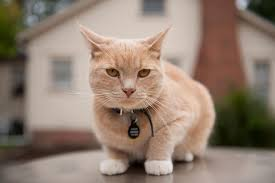
\includegraphics{images/cat.jpg}
  \caption{Cute cat}
  \label{fig:cute_cat}
\end{figure}

Figure \ref{fig:cute_cat} shows one cute cat.

\begin{figure}[ht!]
  \centering
  \begin{subfigure}[b]{0.4\linewidth}
    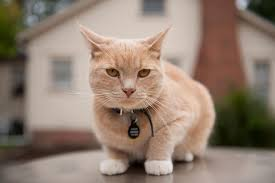
\includegraphics[width=\linewidth]{images/cat.jpg}
    \caption{Left cat.}
  \end{subfigure}
  \begin{subfigure}[b]{0.4\linewidth}
    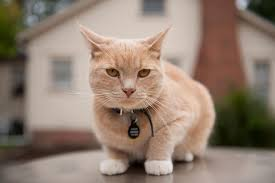
\includegraphics[width=\linewidth]{images/cat.jpg}
    \caption{Right cat.}
  \end{subfigure}
  \caption{The same cute cat. Two times.}
  \label{fig:two_cats}
\end{figure}


\begin{figure}[ht!]

  \centering
  \begin{subfigure}[b]{0.2\linewidth}
    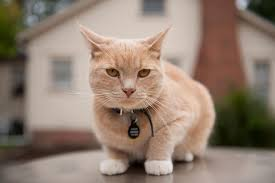
\includegraphics[width=\linewidth]{images/cat.jpg}
     \caption{Left cat.}
  \end{subfigure}
  \begin{subfigure}[b]{0.2\linewidth}
    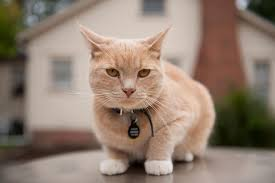
\includegraphics[width=\linewidth]{images/cat.jpg}
    \caption{Middle cat.}
  \end{subfigure}
  \begin{subfigure}[b]{0.2\linewidth}
    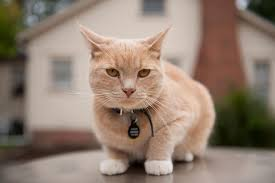
\includegraphics[width=\linewidth]{images/cat.jpg}
    \caption{Right cat.}
  \end{subfigure}

  \begin{subfigure}[b]{0.5\linewidth}
    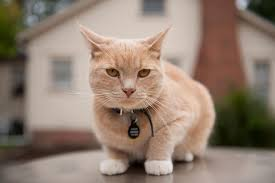
\includegraphics[width=\linewidth]{images/cat.jpg}
    \caption{Big cat.}
  \end{subfigure}

  \caption{The same cute cat. Multiple times.}
  \label{fig:multiple_cats}
\end{figure}
\chapter{Formula}
Formula $f(x) = x^2$ is an example of embeded formula.

Equation:
\begin{equation*}
  1 + 2 = 3
\end{equation*}

Lined formulas for showing solving by step:
\begin{align*}
  1 + 2 &= 3\\
  1 &= 3 - 2
\end{align*}

Fractions:
\begin{align*}
  f(x) &= x^2\\
  g(x) &= \frac{1}{x}\\
  F(x) &= \int^a_b \frac{1}{3}x^3 \mathrm{d}x\\
  G(x) &= \int^4_{-\infty} \frac{1}{3}x^3 \mathrm{d}x\\
  G(x) &= \int^{\frac{\pi}{2}}_{\frac{-\pi}{2}} \frac{1}{3}x^3 \mathrm{d}x
\end{align*}

\begin{equation*}
  \left(
    \frac{1}{\sqrt{x}}
  \right)
\end{equation*}

Sqrt:
\begin{equation*}
  \frac{1}{\sqrt{x}}
\end{equation*}

Matrices:
\begin{equation*}
  \begin{matrix}
  1 & 0\\
  0 & 1
  \end{matrix}
\end{equation*}
\begin{equation*}
\left[
  \begin{matrix}
  1 & 0\\
  0 & 1
  \end{matrix}
\right]
\end{equation*}
\chapter{Kod}

\begin{python}
def func(arg1, arg2):
  print(f"arg1 is {arg1}")
  print(f"arg2 is {arg2}")

class Klasa(SuperClass):
  
  # Class value
  value = 0

  def __init__(self):
    print("Init")

  def inc(self, inc):
    self.value += inc
\end{python}

Inlined python code \pyth{print("Inlined python!")}
\chapter{Zaključak}
Zaključak.

\bibliography{literatura}
\bibliographystyle{fer}

\begin{sazetak}
Sažetak na hrvatskom jeziku.

\kljucnerijeci{lokalizacija, simulacija}
\end{sazetak}

% TODO: Navedite naslov na engleskom jeziku.
\engtitle{Title}
\begin{abstract}
Abstract.

\keywords{simulation, localization.}
\end{abstract}

\end{document}
